% !TeX program = xelatex
\documentclass[UTF8,12pt,a4paper]{ctexart}
\usepackage{amsmath,amssymb}
\usepackage{geometry}
\usepackage{tikz} % 引入绘图包以生成函数图像
\geometry{margin=2cm}

% ===== 水印：贺昱琪学习资料 =====
\usepackage{xcolor}
\usepackage{eso-pic}
\usepackage{graphicx}

\newcommand{\WMText}{贺昱琪学习资料}
\newcommand{\WMScale}{2.28}
\newcommand{\WMAngle}{45}
\colorlet{WMColor}{black!8}

\AddToShipoutPictureBG{%
  \AtPageLowerLeft{%
    \put(\LenToUnit{0.66\paperwidth},\LenToUnit{0.70\paperheight}){%
      \rotatebox{\WMAngle}{\scalebox{\WMScale}{\textcolor{WMColor}{\WMText}}}%
    }%
    \put(\LenToUnit{0.33\paperwidth},\LenToUnit{0.50\paperheight}){%
      \rotatebox{\WMAngle}{\scalebox{\WMScale}{\textcolor{WMColor}{\WMText}}}%
    }%
    \put(\LenToUnit{0.66\paperwidth},\LenToUnit{0.30\paperheight}){%
      \rotatebox{\WMAngle}{\scalebox{\WMScale}{\textcolor{WMColor}{\WMText}}}%
    }%
  }%
}

% ===== 5题铺满一页布局 =====
\usepackage{enumitem}
\newcommand{\BottomWriteSpace}{1.5cm}

\newenvironment{OnePageFiveFill}{
  \small
  \vspace*{0pt}
  \begin{enumerate}[leftmargin=*, itemsep=0pt, topsep=0pt, parsep=0pt, partopsep=0pt]
  \setlength{\parskip}{0pt}
}{
  \end{enumerate}
  \vspace*{\BottomWriteSpace}
  \normalsize
  \newpage
}

\newcommand{\Q}[1]{\item #1\par\vfill}
\newcommand{\Qlast}[1]{\item #1\par}

\begin{document}

% =========================================================
% 5.18
% =========================================================
\section*{5月18日作业（5道题当晚22:00前打卡）}
\begin{OnePageFiveFill}

\Q{计算：$1999 \div 1999\dfrac{1999}{2000}$}

\Q{（相遇问题）在环形跑道上，小明和小华同时从同一地点同向而行，每隔 12 分钟小明就可以追上小华一次。若两人在原地同时出发，相背而行，则每隔 4 分钟就相遇一次。两人跑一圈各需几分钟？}

\Q{（变量间关系）一条公路上依次有 A, B, C 三地，甲车从 A 地出发，沿公路经 B 地到 C 地，乙车从 C 地出发，沿公路驶向 B 地。甲、乙两车同时出发，匀速行驶，乙车比甲车早 $\dfrac{2}{7}$ 时到达目的地。甲、乙两车之间的路程 $y$ (km) 与两车行驶时间 $x$ (h) 的关系如图所示，请结合图象信息，解答下列问题：\\
(1) 求甲车行驶的速度。\\
(2) 求 A, C 两地的距离。\\
(3) 两车出发多少时，乙车距 B 地的路程是甲车距 B 地路程的 3 倍？
\vspace{-0.5em}
\begin{center}
\begin{tikzpicture}[scale=0.85, x=1.5cm, y=0.015cm]
\draw[->] (-0.2,0) -- (5.5,0) node[right] {$x/\mathrm{h}$};
\draw[->] (0,-10) -- (0,350) node[above] {$y/\mathrm{km}$};
\node[below left] at (0,0) {0};
\draw (2.5,0) node[below] {$\frac{5}{2}$} -- (2.5,5);
\draw (4,0) node[below] {$4$} -- (4,5);
\draw (0,180) node[left] {$180$} -- (0.05,180);
\draw (0,200) node[left] {$200$} -- (0.05,200);
\draw[thick] (0,300) node[right]{$D$} -- (2.5,0) node[above]{$E$} -- (4,180) node[left]{$F$} -- (4.28,200) node[above]{$M$};
\draw[dashed] (4,0) -- (4,180) -- (0,180);
\draw[dashed] (4.28,0) -- (4.28,200) -- (0,200);
\end{tikzpicture}
\end{center}}

\Q{（圆锥的体积）一个倒置的圆锥形容器中装有 $5$ 升水，此时水面高度正好是圆锥高度的 $\dfrac{1}{3}$，这个容器还能装水多少升？}

\Qlast{解方程：$\dfrac{4x+3}{3} - \dfrac{3x-1}{2} = \dfrac{x+5}{6}$}

\end{OnePageFiveFill}

% =========================================================
% 5.19
% =========================================================
\section*{5月19日作业（5道题当晚22:00前打卡）}
\begin{OnePageFiveFill}

\Q{计算：$2024 \div 2024\dfrac{2024}{2025}$}

\Q{（相遇问题）在环形跑道上，小明和小华同时从同一地点同向而行，每隔 18 分钟小明就可以追上小华一次。若两人在原地同时出发，相背而行，则每隔 6 分钟就相遇一次。两人跑一圈各需几分钟？}

\Q{（变量间关系）一条公路上依次有 A, B, C 三地，甲车从 A 地出发，沿公路经 B 地到 C 地，乙车从 C 地出发，沿公路驶向 B 地。甲、乙两车同时出发，匀速行驶，乙车比甲车早 $1$ 时到达目的地。甲、乙两车之间的路程 $y$ (km) 与两车行驶时间 $x$ (h) 的关系如图所示，请结合图象信息，解答下列问题：\\
(1) 求甲车行驶的速度。\\
(2) 求 A, C 两地的距离。\\
(3) 两车出发多少时，乙车距 B 地的路程是甲车距 B 地路程的 3 倍？
\vspace{-0.5em}
\begin{center}
\begin{tikzpicture}[scale=0.85, x=1.5cm, y=0.015cm]
\draw[->] (-0.2,0) -- (6.5,0) node[right] {$x/\mathrm{h}$};
\draw[->] (0,-10) -- (0,350) node[above] {$y/\mathrm{km}$};
\node[below left] at (0,0) {0};
\draw (3,0) node[below] {$3$} -- (3,5);
\draw (4,0) node[below] {$4$} -- (4,5);
\draw (0,100) node[left] {$100$} -- (0.05,100);
\draw (0,160) node[left] {$160$} -- (0.05,160);
\draw[thick] (0,300) node[right]{$D$} -- (3,0) node[above]{$E$} -- (4,100) node[left]{$F$} -- (5,160) node[above]{$M$};
\draw[dashed] (4,0) -- (4,100) -- (0,100);
\draw[dashed] (5,0) -- (5,160) -- (0,160);
\end{tikzpicture}
\end{center}}

\Q{（圆锥的体积）一个倒置的圆锥形容器中装有 $2$ 升水，此时水面高度正好是圆锥高度的 $\dfrac{1}{2}$，这个容器还能装水多少升？}

\Qlast{解含方程：$\dfrac{1.6x-0.8}{0.4} - \dfrac{1.2x+3}{0.6} = 5$}

\end{OnePageFiveFill}

% =========================================================
% 5.20
% =========================================================
\section*{5月20日作业（5道题当晚22:00前打卡）}
\begin{OnePageFiveFill}

\Q{计算：$99 \div 99\dfrac{99}{100}$}

\Q{（相遇问题）在环形跑道上，小明和小华同时从同一地点同向而行，每隔 24 分钟小明就可以追上小华一次。若两人在原地同时出发，相背而行，则每隔 8 分钟就相遇一次。两人跑一圈各需几分钟？}

\Q{（变量间关系）一条公路上依次有 A, B, C 三地，甲车从 A 地出发，沿公路经 B 地到 C 地，乙车从 C 地出发，沿公路驶向 B 地。甲、乙两车同时出发，匀速行驶，乙车比甲车早 $\dfrac{1}{4}$ 时到达目的地。甲、乙两车之间的路程 $y$ (km) 与两车行驶时间 $x$ (h) 的关系如图所示，请结合图象信息，解答下列问题：\\
(1) 求甲车行驶的速度。\\
(2) 求 A, C 两地的距离。\\
(3) 两车出发多少时，乙车距 B 地的路程是甲车距 B 地路程的 3 倍？
\vspace{-0.5em}
\begin{center}
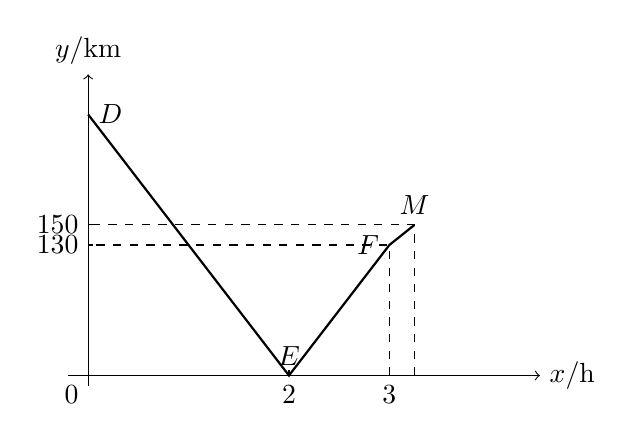
\begin{tikzpicture}[scale=0.85, x=1.5cm, y=0.015cm]
\draw[->] (-0.2,0) -- (4.5,0) node[right] {$x/\mathrm{h}$};
\draw[->] (0,-10) -- (0,300) node[above] {$y/\mathrm{km}$};
\node[below left] at (0,0) {0};
\draw (2,0) node[below] {$2$} -- (2,5);
\draw (3,0) node[below] {$3$} -- (3,5);
\draw (0,130) node[left] {$130$} -- (0.05,130);
\draw (0,150) node[left] {$150$} -- (0.05,150);
\draw[thick] (0,260) node[right]{$D$} -- (2,0) node[above]{$E$} -- (3,130) node[left]{$F$} -- (3.25,150) node[above]{$M$};
\draw[dashed] (3,0) -- (3,130) -- (0,130);
\draw[dashed] (3.25,0) -- (3.25,150) -- (0,150);
\end{tikzpicture}
\end{center}}

\Q{（圆锥的体积）一个倒置的圆锥形容器中装有 $1$ 升水，此时水面高度正好是圆锥高度的 $\dfrac{1}{3}$，这个容器还能装水多少升？}

\Qlast{解方程：$\dfrac{2x+1}{4} - \dfrac{x-3}{3} = \dfrac{x}{2} + 1$}

\end{OnePageFiveFill}

% =========================================================
% 5.21
% =========================================================
\section*{5月21日作业（5道题当晚22:00前打卡）}
\begin{OnePageFiveFill}

\Q{计算：$100 \div 100\dfrac{100}{101}$}

\Q{（相遇问题）在环形跑道上，小明和小华同时从同一地点同向而行，每隔 30 分钟小明就可以追上小华一次。若两人在原地同时出发，相背而行，则每隔 10 分钟就相遇一次。两人跑一圈各需几分钟？}

\Q{（变量间关系）一条公路上依次有 A, B, C 三地，甲车从 A 地出发，沿公路经 B 地到 C 地，乙车从 C 地出发，沿公路驶向 B 地。甲、乙两车同时出发，匀速行驶，乙车比甲车早 $\dfrac{11}{5}$ 时到达目的地。甲、乙两车之间的路程 $y$ (km) 与两车行驶时间 $x$ (h) 的关系如图所示，请结合图象信息，解答下列问题：\\
(1) 求甲车行驶的速度。\\
(2) 求 A, C 两地的距离。\\
(3) 两车出发多少时，乙车距 B 地的路程是甲车距 B 地路程的 3 倍？
\vspace{-0.5em}
\begin{center}
\begin{tikzpicture}[scale=0.85, x=1.5cm, y=0.015cm]
\draw[->] (-0.2,0) -- (8.5,0) node[right] {$x/\mathrm{h}$};
\draw[->] (0,-10) -- (0,400) node[above] {$y/\mathrm{km}$};
\node[below left] at (0,0) {0};
\draw (4,0) node[below] {$4$} -- (4,5);
\draw (5,0) node[below] {$5$} -- (5,5);
\draw (0,90) node[left] {$90$} -- (0.05,90);
\draw (0,200) node[left] {$200$} -- (0.05,200);
\draw[thick] (0,360) node[right]{$D$} -- (4,0) node[above]{$E$} -- (5,90) node[left]{$F$} -- (7.2,200) node[above]{$M$};
\draw[dashed] (5,0) -- (5,90) -- (0,90);
\draw[dashed] (7.2,0) -- (7.2,200) -- (0,200);
\end{tikzpicture}
\end{center}}

\Q{（圆锥的体积）一个倒置的圆锥形容器中装有 $6$ 升水，此时水面高度正好是圆锥高度的 $\dfrac{1}{2}$，这个容器还能装水多少升？}

\Qlast{解含方程：$\dfrac{1.5x-0.5}{0.5} - \dfrac{2x+1}{0.2} = -2$}

\end{OnePageFiveFill}

% =========================================================
% 5.22
% =========================================================
\section*{5月22日作业（5道题当晚22:00前打卡）}
\begin{OnePageFiveFill}

\Q{计算：$999 \div 999\dfrac{999}{1000}$}

\Q{（相遇问题）在环形跑道上，小明和小华同时从同一地点同向而行，每隔 36 分钟小明就可以追上小华一次。若两人在原地同时出发，相背而行，则每隔 12 分钟就相遇一次。两人跑一圈各需几分钟？}

\Q{（变量间关系）一条公路上依次有 A, B, C 三地，甲车从 A 地出发，沿公路经 B 地到 C 地，乙车从 C 地出发，沿公路驶向 B 地。甲、乙两车同时出发，匀速行驶，乙车比甲车早 $\dfrac{1}{3}$ 时到达目的地。甲、乙两车之间的路程 $y$ (km) 与两车行驶时间 $x$ (h) 的关系如图所示，请结合图象信息，解答下列问题：\\
(1) 求甲车行驶的速度。\\
(2) 求 A, C 两地的距离。\\
(3) 两车出发多少时，乙车距 B 地的路程是甲车距 B 地路程的 3 倍？
\vspace{-0.5em}
\begin{center}
\begin{tikzpicture}[scale=0.85, x=1.5cm, y=0.015cm]
\draw[->] (-0.2,0) -- (4.5,0) node[right] {$x/\mathrm{h}$};
\draw[->] (0,-10) -- (0,350) node[above] {$y/\mathrm{km}$};
\node[below left] at (0,0) {0};
\draw (2,0) node[below] {$2$} -- (2,5);
\draw (3,0) node[below] {$3$} -- (3,5);
\draw (0,150) node[left] {$150$} -- (0.05,150);
\draw (0,180) node[left] {$180$} -- (0.05,180);
\draw[thick] (0,300) node[right]{$D$} -- (2,0) node[above]{$E$} -- (3,150) node[left]{$F$} -- (3.33,180) node[above]{$M$};
\draw[dashed] (3,0) -- (3,150) -- (0,150);
\draw[dashed] (3.33,0) -- (3.33,180) -- (0,180);
\end{tikzpicture}
\end{center}}

\Q{（圆锥的体积）一个倒置的圆锥形容器中装有 $3$ 升水，此时水面高度正好是圆锥高度的 $\dfrac{1}{2}$，这个容器还能装水多少升？}

\Qlast{解方程：$\dfrac{3x-2}{5} + \dfrac{x+1}{2} = x + 1.4$}

\end{OnePageFiveFill}

% =========================================================
% 5.23
% =========================================================
\section*{5月23日作业（5道题当晚22:00前打卡）}
\begin{OnePageFiveFill}

\Q{计算：$50 \div 50\dfrac{50}{51}$}

\Q{（相遇问题）在环形跑道上，小明和小华同时从同一地点同向而行，每隔 15 分钟小明就可以追上小华一次。若两人在原地同时出发，相背而行，则每隔 5 分钟就相遇一次。两人跑一圈各需几分钟？}

\Q{（变量间关系）一条公路上依次有 A, B, C 三地，甲车从 A 地出发，沿公路经 B 地到 C 地，乙车从 C 地出发，沿公路驶向 B 地。甲、乙两车同时出发，匀速行驶，乙车比甲车早 $1$ 时到达目的地。甲、乙两车之间的路程 $y$ (km) 与两车行驶时间 $x$ (h) 的关系如图所示，请结合图象信息，解答下列问题：\\
(1) 求甲车行驶的速度。\\
(2) 求 A, C 两地的距离。\\
(3) 两车出发多少时，乙车距 B 地的路程是甲车距 B 地路程的 3 倍？
\vspace{-0.5em}
\begin{center}
\begin{tikzpicture}[scale=0.85, x=1.5cm, y=0.015cm]
\draw[->] (-0.2,0) -- (6.5,0) node[right] {$x/\mathrm{h}$};
\draw[->] (0,-10) -- (0,450) node[above] {$y/\mathrm{km}$};
\node[below left] at (0,0) {0};
\draw (3,0) node[below] {$3$} -- (3,5);
\draw (4,0) node[below] {$4$} -- (4,5);
\draw (0,125) node[left] {$125$} -- (0.05,125);
\draw (0,200) node[left] {$200$} -- (0.05,200);
\draw[thick] (0,375) node[right]{$D$} -- (3,0) node[above]{$E$} -- (4,125) node[left]{$F$} -- (5,200) node[above]{$M$};
\draw[dashed] (4,0) -- (4,125) -- (0,125);
\draw[dashed] (5,0) -- (5,200) -- (0,200);
\end{tikzpicture}
\end{center}}

\Q{（圆锥的体积）一个倒置的圆锥形容器中装有 $4$ 升水，此时水面高度正好是圆锥高度的 $\dfrac{1}{3}$，这个容器还能装水多少升？}

\Qlast{解方程：$\dfrac{5x-1}{6} - \dfrac{2x+3}{4} = \dfrac{x-3}{2}$}

\end{OnePageFiveFill}

\end{document}